\chapter{Estadística de Tsallis}\label{ch-Tsallis}

% \pagestyle{fancy}
% \fancyhead{} % clear all header fields
% \fancyhead[RO,LE]{\textbf{\chaptername\,\thechapter}  }
% \fancyfoot{} % clear all footer fields
% \fancyfoot[LE,RO]{\thepage}
% % \fancyfoot[LO,CE]{Introducción}
% \fancyfoot[CO,CE]{Estadística de Tsallis}

\section{Introducción}

La mecánica estadística estándar está basada en la entropía de \acrfull{bg}, 

\begin{equation}
{S}_{\mathrm{BG}} = - k \sum_{i=1}^{W} {p}_{i} \ln {p}_{i}, \quad \sum_{i=1}^{W} {p}_{i} = 1
\end{equation}

donde $W$ es el número de configuraciones microscópicas del sistema y ${p}_{i}$ es la probabilidad de acceder a la $i$-ésima configuración. Sin embargo, sistemas de no lineales dinámicos de muchos cuerpos requieren \emph{ergodicidad} (que su valor esperado sea igual a su promedio a largo plazo). Para sistemas no ergódicos, que sucede con sistemas complejos, no existe razón para usar estadística \acrshort{bg}. Por esta razón se ha requerido de una extensión para sistemas de este tipo, llamados \emph{no extensivos} (pues no son proporcional al número total de elementos del sistema), una de ellas es la siguiente, que extiende la entropía de \acrshort{bg} como

\begin{equation}
{S}_{q} = k \frac{1-\sum_{i} {p}_{i}^{q}}{q-1} \qquad (q\in \mathbb{R};\; {S}_{q=1} = {S}_{\mathrm{BG}})
\end{equation}

Bajo esta generalización, en un sistema constituido por dos subsistemas probabilisticamente independientes $A$ y $B$ (i.e., si ${p}_{ij}^{A+B} = {p}_{i}^{A}{p}_{j}^{B}$), entonces

\begin{equation}\label{eq-TsallisTwoSystems}
\frac{{S}_{{q}}(A+B)}{k} = \frac{{S}_{q}(A)}{k} + \frac{{S}_{q}(B)}{k} + (1 - q) \frac{{S}_{q}(A)}{k}\frac{{S}_{q}(B)}{k},
\end{equation}

(más adelante se usarán unidades naturales por lo que no aparecerá la constante de \acrshort{bg}, $k$) de donde se observa claramente que cuando $q=1$ se regresa a la estadística de \acrshort{bg} [ref Tsallis statistics].

NOTA: En la misma referencia se agrega la obtención de la energía de Tsallis para las masas

\section{Presión dentro del hadrón}\label{sec-PresTsa}

A partir de la ecuación \eqref{eq-TsallisTwoSystems}, podemos obtener la entropía dentro de un hadrón que consiste en una mezcla de gases quarks y gluon. De esta manera empezamos por considerar el cálculo de cada contribución, los quarks vistos como un gas ideal de Fermi ultrarelativista y los gluones vistos como un gas ideal de \acrfull{be}  ultrarelativista, ambos sin masa y no interactuantes, la interacción vendrá al final del parámetro $q$ de Tsallis

\subsection{Presión de gluones, un gas ideal de Bose - Einstein ultrarelativista}

Los níveles de energía de un bosón visto como un gas ideal de \acrshort{be} están dados por ${\epsilon}_{k}=cp=\hbar c k$, $p$ es la magnitud del momento de las partículas del gas, y $k$ la magnitud del vector de onda. Y la función de partición para un gas ideal de \acrshort{be} está determinada por:

\begin{equation}\label{eq-partfunc}
{\Xi}^{\mathrm{BE}}\left(T,V,\mu\right) = \prod_{k=1}^{\infty}\frac{1}{1-\xi {e}^{-\beta {\epsilon}_{k}}},
\end{equation}

donde $\beta = \frac{1}{kT}$, y ${\xi} = {e}^{\beta \mu}$ es la fugacidad del gas, $T$ es la temperatura del gas, $V$ el volumen del gas y $\mu$ el potencial químico del gas. El número de partículas promedio en cada estado de energía ${\epsilon}_{k}$ se calcula a través de la ecuación:

\begin{equation}\label{eq-avg-numb-parts}
\left\langle {n}_{k} \right\rangle = -\frac{1}{\beta} \frac{\partial}{\partial {\epsilon}_{k}} \ln {\Xi}^{\mathrm{BE}}\left.\right|_{\xi,V,{\epsilon}_{i \neq k}},
\end{equation}

\begin{equation}
\left\langle {n}_{k} \right\rangle = \frac{1}{{\xi}^{-1}{e}^{\beta{\epsilon}_{k}}-1} 
\end{equation}

De tal manera que el número total de partículas promedio y energía se pueden calcular como

\begin{equation}\label{eq-BE-Ntotal}
N(T,V,\mu)=\sum_{k}\left\langle {n}_{k} \right\rangle = \sum_{k}\frac{1}{{\xi}^{-1}{e}^{\beta{\epsilon}_{k}}-1}
\end{equation}

\begin{equation}\label{eq-BE-Etotal}
E(T,V,\mu) = \sum_{k}\left\langle {n}_{k} \right\rangle {\epsilon}_{k} = \sum_{k}\frac{{\epsilon}_{k}}{{\xi}^{-1}{e}^{\beta{\epsilon}_{k}}-1}.
\end{equation}

Para una gran cantidad de partículas, podemos sustituir la suma por una integral, considerando el número total de estados en el espacio fase clásico tenemos

\begin{equation}
\begin{split}
\Sigma &= \int \frac{\mathrm{d}^{3}r \mathrm{d}^{3}p}{{h}^{3}} \\ 
& = V\int \frac{4\pi {p}^{2} \mathrm{d}p}{{h}^{3}} \\
& = \frac{4\pi V}{{h}^{3}} \int_{0}^{\infty} {p}^{2} \mathrm{d} p 
\end{split}
\end{equation}

Usando la relación ${\epsilon}_{k} = cp$ obtenemos

\begin{equation}\label{eq-totalestados}
\Sigma = \frac{4\pi V}{(hc)^{3}} \int_{0}^{\infty} {\epsilon}^{2} \mathrm{d} \epsilon
\end{equation} 

De esta forma, sustituyendo \eqref{eq-totalestados} en \eqref{eq-BE-Ntotal} y \eqref{eq-BE-Etotal}, obtenemos

\begin{equation}\label{eq-BE-Ntotalint}
N(T,V,\mu) = \frac{4\pi V}{(hc)^{3}} \int_{0}^{\infty} \frac{{\epsilon}^{2} \mathrm{d} \epsilon}{{\xi}^{-1} {e}^{\beta \epsilon} - 1}
\end{equation}

\begin{equation}\label{eq-BE-Etotalint}
E(T,V,\mu) = \frac{4\pi V}{(hc)^{3}} \int_{0}^{\infty} \frac{{\epsilon}^{3} \mathrm{d} \epsilon}{{\xi}^{-1} {e}^{\beta \epsilon} - 1}
\end{equation}

Dado que tratamos con partículas sin masa, es posible tener infinitas partículas con energía ${\epsilon}_{0}=0$. De esta manera, el potencial químico $\mu$ debe ser cero pues es posible crear infinitas partículas con energía $0$ sin afectar a nuestros resultados puesto que no contribuyen a la energía total del sistema. Así, si $\mu=0$, entonces $\xi = 1$. Y sustituyendo en las ecuaciones \eqref{eq-BE-Ntotalint} y \eqref{eq-BE-Etotalint} obtenemos 

\begin{equation}\label{eq-BE-Ntotalintnofug}
N(T,V) = \frac{4\pi V}{(hc)^{3}} \int_{0}^{\infty} \frac{{\epsilon}^{2} \mathrm{d} \epsilon}{{e}^{\beta \epsilon} - 1}
\end{equation}

\begin{equation}\label{eq-BE-Etotalintnofug}
E(T,V) = \frac{4\pi V}{(hc)^{3}} \int_{0}^{\infty} \frac{{\epsilon}^{3} \mathrm{d} \epsilon}{ {e}^{\beta \epsilon} - 1}
\end{equation}

Para resolver las integrales, consideramos el cambio de variable $x=\beta \epsilon$, por lo que $\epsilon = \frac{x}{\beta}$ y así $\mathrm{d}\epsilon = \frac{\mathrm{d}x}{\beta}$ y así, entonces 

\begin{equation}\label{eq-BE-Ntotalintnofug-x}
N(T,V) = \frac{4\pi V}{(hc)^{3}} \frac{1}{{\beta}^{3}}\int_{0}^{\infty} \frac{{x}^{2} \mathrm{d} x}{{e}^{x} - 1}
\end{equation}

\begin{equation}\label{eq-BE-Etotalintnofug-x}
E(T,V) = \frac{4\pi V}{(hc)^{3}} \frac{1}{{\beta}^{4}} \int_{0}^{\infty} \frac{{x}^{3} \mathrm{d} x}{ {e}^{x} - 1}
\end{equation}

Con lo cual, obtenemos las funciones especiales ${g}_{n}(\xi)$ con $0 \leq \xi \leq 1$ tales que

\begin{equation}\label{eq-g-xi}
{g}_{n}(\xi) = \frac{1}{\Gamma(n)} \int_{0}^{\infty} \frac{{x}^{n-1} \mathrm{d}x}{{\xi}^{-1}{e}^{x}-1}
\end{equation}

Tal que las integrales de \eqref{eq-BE-Ntotalintnofug-x} y \eqref{eq-BE-Etotalintnofug-x} se vuelven

\begin{equation}\label{eq-sol-int-N}
\int_{0}^{\infty} \frac{{x}^{2} \mathrm{d} x}{ {e}^{x} - 1} = \Gamma(3) {g}_{3}(1)
\end{equation}

\begin{equation}\label{eq-sol-int-E}
\int_{0}^{\infty} \frac{{x}^{3} \mathrm{d} x}{ {e}^{x} - 1}= \Gamma(4) {g}_{4}(1)
\end{equation}

Sustituyendo las ecuaciones \eqref{eq-sol-int-N} y \eqref{eq-sol-int-E} en \eqref{eq-BE-Ntotalintnofug-x} y \eqref{eq-BE-Etotalintnofug-x}, respectivamente, y usando la propiedad ${g}_{n}(1) = \zeta(n)$, con $\zeta(n)$ representando la función zeta de Rienamann, se obtiene

\begin{equation}\label{eq-BE-Ntotalintreduced1}
N(T,V) = \frac{4\pi V}{(hc)^{3}} \frac{1}{{\beta}^{3}}\Gamma(3) \zeta(3)
\end{equation}

\begin{equation}\label{eq-BE-Etotalintreduced1}
E(T,V) = \frac{4\pi V}{(hc)^{3}} \frac{1}{{\beta}^{4}} \Gamma(4) \zeta(4)
\end{equation}

Ya que $\Gamma(n-1) = n!$ y $\zeta(4) = \frac{{\pi}^{4}}{90}$ se llega a

 \begin{equation}\label{eq-BE-Ntotalintreduced2}
N(T,V) = 8\pi V \left(\frac{kT}{hc} \right)^{3} \zeta(3)
\end{equation}

\begin{equation}\label{eq-BE-Etotalintreduced2}
E(T,V) = \frac{8\pi V}{(hc)^{3}} \left(k T \right)^{4} \frac{{\pi}^{4}}{30}
\end{equation}

Y usando unidades naturales $\hbar=k=x=1$ y $h=2\pi \hbar = 2\pi$, así entonces

 \begin{equation}\label{eq-BE-Ntotalintreduced3}
N(T,V) = \frac{1}{{\pi}^{2}} \zeta(3)V{T}^{3}
\end{equation}

\begin{equation}\label{eq-BE-Etotalintreduced3}
E(T,V) = \frac{{\pi}^{2}}{30} V{T}^{4}
\end{equation}

Finalmente, dado que hay tres componentes independientes de la carga de color, y consecuentemente $3 \times 3 - 1$ generadores de $SU(3)$, hay 8 diferentes tipos de gluones, y como cada gluón tiene dos proyecciones de espín, el factor de degeneración corresponde a ${g}_{G} = 8 \times 2 = 16$. Por lo tanto, pasamos a que las expresiones para el número total de gluones y la energía total de gluones como un gas ideal de \acrshort{be} ultrarrelativista son

 \begin{equation}\label{eq-BE-Ntotalgluons}
{N}_{G}(T,V) = \frac{{g}_{G}}{{\pi}^{2}} \zeta(3)V{T}^{3}
\end{equation}

\begin{equation}\label{eq-BE-Etotalgluons}
{E}_{G}(T,V) = {g}_{G}\frac{{\pi}^{2}}{30} V{T}^{4}
\end{equation}

Para calcular la contribución de presión debido a los gluones, partimos de la función de partición ${\Xi}^{BE}$ y el potencial macrocanónico o potencial gran canónico $\phi$

\begin{equation}\label{eq-BE-P1}
\begin{split}
\phi = -PV  & = -k T \ln {\Xi}^{BE} \\ 
\Rightarrow P & = \frac{kT}{V} \ln {\Xi}^{BE}
\end{split}
\end{equation}

Calculando el logaritmo de la función de partición \eqref{eq-partfunc} se tiene

\begin{equation}
\ln {\Xi}^{BE} = - \sum_{k=1}^{\infty} \ln\left(1 - \xi{e}^{-\beta {\epsilon}_{k}}\right)
\end{equation}

Nuevamente ocupamos el hecho de que son estados energéticos tan cercanos y tal cantidad de partículas en distintos estados energéticos, podemos sustituir la suma por una integral, usando el número total de estados \eqref{eq-totalestados} y el hecho de que no hay potencial químico ($\mu=0 \Rightarrow \xi=1$) para obtener

\begin{equation}
\ln {\Xi}^{BE} = - \frac{4\pi V}{(hc)^{3}} \int_{0}^{\infty} {\epsilon}^{2} \ln \left(1 - {e}^{-\beta\epsilon} \right) \mathrm{d} \epsilon
\end{equation}

Realizando la integral por partes tendremos

\begin{equation}
\begin{split}
\ln {\Xi}^{BE} & = - \frac{4\pi V}{(hc)^{3}} \left[ \left. \frac{1}{3} {\epsilon}^{3} \ln \left( 1 - {e}^{-\beta \epsilon}\right) \right|_{0}^{\infty} - \frac{1}{3} \beta \int_{0}^{\infty} \frac{{\epsilon}^{3} \mathrm{d}\epsilon}{{e}^{\beta \epsilon} - 1} \right] \\ 
& = \frac{4\pi V}{(hc)^{3}} \frac{kT}{3} \int_{0}^{\infty} \frac{{\epsilon}^{3} \mathrm{d} \epsilon}{{e}^{-\beta \epsilon} - 1}
\end{split}
\end{equation}

Resolviendo la integral, de la misma forma que con la ecuación \eqref{eq-BE-Etotalintnofug}, usando \eqref{eq-sol-int-E} y simplificando se llega a que la presión ejercida por un gas de partículas ultrarrelativistas tipo \acrshort{be}, usando la expresión \eqref{eq-BE-P1}, está dada como

\begin{equation}\label{eq-BE-P2}
P= \frac{1}{3} \frac{E}{V}
\end{equation}

Y dado que existen ${g}_{G}$ estados degenerados para la energía de los gluones, entonces, la presión correspondiente a los gluones es, usando \eqref{eq-BE-Etotalgluons},

\begin{equation}\label{eq-BE-Pgluons}
{P}_{G} = {g}_{G} \frac{{\pi}^{2}}{90}{T}^{4}
\end{equation}

Como cálculo final, hallamos la entropía a partir del potencial gran canónico por medio de la relación

\begin{equation}\label{eq-BE-Entropy}
\begin{split}
\phi &= E-TS-\mu N = -PV, \\
\Rightarrow S & = \frac{1}{T} \left(E+PV- \mu N \right)
\end{split}
\end{equation}

Sustituyendo la ecuación \eqref{eq-BE-P2} en \eqref{eq-BE-Entropy} y considerando $\mu=0$, la entropía del sistema es

\begin{equation}\label{eq-BE-S}
S = \frac{4}{3} \frac{E}{T}
\end{equation}

Y tomando en cuenta que tratamos con la energía de gluones \eqref{eq-BE-Etotalgluons}, la entropía del gas de gluones está dado como

\begin{equation}\label{eq-BE-Sgluons}
{S}_{G} = 4{g}_{G} \frac{{\pi}^{2}}{90}V{T}^{3}.
\end{equation}

\subsection{Presión de quarks, un gas ideal de Fermi - Dirac ultrarrelativista}\label{sec-Pquarks}

Las partículas ultrarelativistas tienen una relación energía-momento $\epsilon = \| \overrightarrow{p} \| c$\footnote{De la fórmula general $\epsilon = \sqrt{{p}^{2}{c}^{2} + {m}^{2}{c}^{4}}$, para masa en reposo despreciable.}.

Hay ciertos bosones con esta relación energía-momento, pero el número de fermiones con masa en reposo despreciable es muy poca. Para casos prácticos, ``despreciable'' significa una masa en reposo del orden de los neutrinos (${m}_{\nu} < 8 $eV). El gas ultrarelativistico de \acrfull{fd} puede ser visto como un gas caliente de fermiones con masa en reposo no despreciable, esto es, si el momento promedio en el gas es grande comparado con $mc$, es decir, si la energía térmica promedio $kT$ es grande comparada con la masa en reposo.

A partir de mecánica cuántica relativista, se sabe que uno puede crear pares de partículas y antipartículas (quarks y antiquarks, en nuestro caso) del vacío con un gasto energético de $2m{c}^{2}$. Por lo tanto, no debemos considerar un gas de partículas \acrshort{fd} solitarias, sino como pares partícula-antipartícula.

Así, trataremos con una mezcla de dos gases ideales \acrshort{fd}, entre las cuales, son posibles reacciones ``químicas''.

La función de partición para un gas ideal de \acrshort{fd}  está determinada por:

\begin{equation}
{\Xi}^{\mathrm{FD}}(T,V,\mu)=\prod_{k=1}^{\infty} \left(1 + \xi {e}^{-\beta {\epsilon}_{k}} \right)
\end{equation}

En este caso se considera una mezcla de gases (quarks y antiquarks), entonces la función de partición está dada como

\begin{equation}
\Xi\left(T,V,{\mu}_{+},{\mu}_{-}\right) = \prod_{{\epsilon}_{+}} \left(1+ {\xi}_{+}{e}^{-\beta {\epsilon}_{+}} \right) + \prod_{{\epsilon}_{-}} \left(1+ {\xi}_{-}{e}^{-\beta {\epsilon}_{-}} \right)
\end{equation}

donde ${\xi}_{+} = {e}^{\beta {\mu}_{+}}$ y ${\xi}_{-} = {e}^{\beta{\mu}_{-}}$ y el signo $+$ corresponde a las partículas mientras que el signo $-$ a las antipartículas. El número promedio de partículas en cada estado de energía se puede calcular usando la ecuación \eqref{eq-avg-numb-parts} y se obtiene

\begin{equation}\label{eq-FD-NumbParts}
\left\langle{n}_{k} \right\rangle = \frac{1}{{\xi}^{-1}{e}^{\beta{\epsilon}_{k}} + 1}
\end{equation}

por lo que el número total promedio para las partículas se calcularía a través de

\begin{equation}\label{eq-FD-Tot-Numb-Parts}
\begin{split}
{N}_{+}(T,V,{\mu}_{+}) &= \sum_{{\epsilon}_{+}} \left\langle{n}_{{\epsilon}_{+}} \right\rangle\\
& = \sum_{{\epsilon}_{+}} \frac{1}{{\xi}_{+}^{-1}{e}^{\beta{{\epsilon}}_{+}} + 1}
\end{split}
\end{equation}

Y de manera análoga se obtiene el número total promedio de antipartículas

\begin{equation}\label{eq-FD-Tot-Numb-Antiparts}
\begin{split}
{N}_{-}(T,V,{\mu}_{-}) &= \sum_{{\epsilon}_{-}} \left\langle{n}_{{\epsilon}_{-}} \right\rangle\\
& = \sum_{{\epsilon}_{-}} \frac{1}{{\xi}_{-}^{-1}{e}^{\beta{{\epsilon}}_{-}} + 1}
\end{split}
\end{equation}

En equilibrio termodinámico el número de promedio de partículas y antipartículas cambia constantemente debido al proceso de creación y aniquilación, por lo que no es conveniente fijar el número de ambas y posteriormente determinar los potenciales químicos. En lugar de ello, se realiza el siguiente análisis a fin de fijar el potencial químico.

Los cambios $d{N}_{+}$ y $d{N}_{-}$ de los dos números de partículas están relacionados por la relación

$$
d{N}_{+} = d{N}_{-}
$$

Las reacciones que suceden en el gas de quarks y antiquarks son de la forma

$$
q + \bar{q} \rightleftharpoons \, \mathrm{productos \; de \; reacci\acute{o}n} + \Delta E
$$

observamos que una antipartícula se crea o aniquila con cada partícula. Además, el resto de las partículas generadas por las reacciones creación-aniquilación no juegan un rol en el gas que estamos considerando de quarks antiquarks. Por esta razón, podemos notar que los potenciales químicos de partículas y antipartículas tienen que ser iguales con signos opuestos, ya que los productos de la reacción no contienen potencial químico,

\begin{equation}\label{eq-FD-chpot-fug}
{\mu}_{+} + {\mu}_{-} = 0, \quad {z}_{+}{z}_{-}=1
\end{equation}

Los números de partículas ${N}_{+}$ y ${N}_{-}$ no son independientes uno de otro, y por lo tanto no hay dos fugacidades independientes, sino en realidad solo uno. Sin embargo, en vez de ${N}_{+}$ y ${N}_{-}$ uno puede fijar la diferencia $N = {N}_{+} - {N}_{-}$, el excedente de partículas, yaa que no está influenciada por los procesos de creación y aniquilación:

\begin{equation}\label{eq-FD-ExcedenteNumParts}
\begin{split}
N & = {N}_{+} - {N}_{-} \\
& = \sum_{{\epsilon}_{+} > 0} \frac{1}{{\xi}_{+}^{-1}{e}^{\beta{{\epsilon}}_{+}} + 1} -\sum_{{\epsilon}_{-} > 0} \frac{1}{{\xi}_{-}^{-1}{e}^{\beta{{\epsilon}}_{-}} + 1}
\end{split}
\end{equation}

A partir de esta ecuación, uno determina la fugacidad tomando en cuenta la ecuación \eqref{eq-FD-chpot-fug}. En este sistema, el excedente $N$ de partículas no cambia por creación-aniquilación, pero el número de partículas medio ${N}_{+}$ y ${N}_{-}$ no puede ser controlado.

\begin{wrapfigure}{l}{0.35\textwidth}
\centering
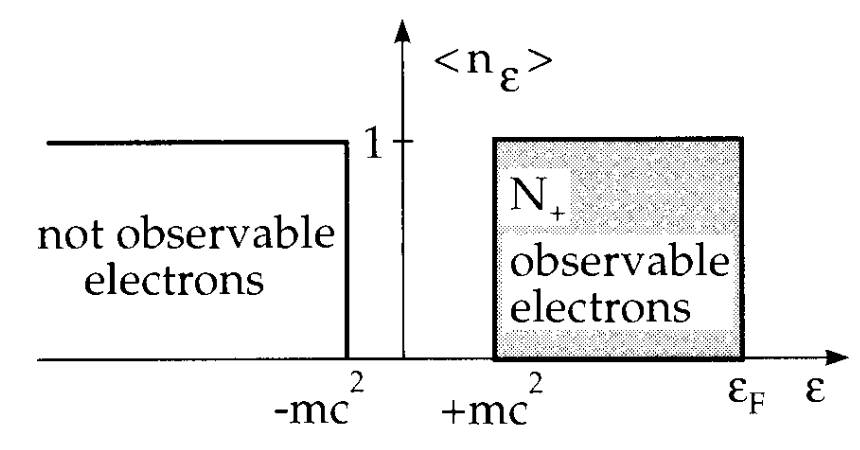
\includegraphics[width=0.35\textwidth]{./Images/ParticleNumberGaswithTnull.png}
\caption[Número de partículas para un gas de electrones a $T=0$]{\emph{$\left\langle {n}_{k} \right\rangle$ para un gas de electrones a $T=0$}}
\label{fig: Gas de electrones}
\end{wrapfigure}

Para explicar lo anterior, tenemos que considerar el espectro de energía de la ecuación libre de Dirac. En el caso ultrarelativista, $m \rightarrow 0$. En este espectro también hay estados de energía $\epsilon \leq -m {c}^{2}$ además de los estados de energía positiva $\epsilon \geq m{c}^{2}$. Uno puede describir ahora partículas y antipartículas en el espectro simultáneamente, si uno asume que en el vacío, sin partículas, todos los estados de energía negativa continua están ocupadas por electrones (inobservables).

En esta imagen de partículas (como son los electrones), en el continuo negativo (agujeros) son interpretados como antipartículas.

Para un gas de electrones con ${N}_{+}$ electrones y una energía de Fermi ${\epsilon}_{\mathrm{FD}} > m{c}^{2}$ tenemos en $T=0$ la situación de la figura \ref{fig: Gas de electrones}.

Si se aumenta la temperatura del gas de electrones, al principio, los electrones cerca de la energía de Fermi son excitados a estados más altos ${\epsilon} > {\epsilon}_{\mathrm{FD}}$. Esto ocurre en un rango de energía de anchura aproximada $kT$ alrededor de la energía de Fermi.

Sin embargo, si la temperatura es del orden de $2m{c}^{2}$, más y más electrones de un continuo más bajo pueden ser excitados en estados libres $\epsilon > {\epsilon}_{\mathrm{FD}}$. Estos electrones dejan huecos en el continuo más bajo, que representan positrones observables. El número de electrones observables también se incrementa. La diferencia ${N}_{+} - {N}_{-}$ sin embargo es la misma que antes. La energía negativa de los huecos ${\epsilon}_{\mathrm{huecos}} < - m{c}^{2}$ es simplemente relacionada a la energía positiva del positrón correspondiente como ${\epsilon}_{{e}^{+}} = - {\epsilon}_{\mathrm{hueco}}$.

El número de electrones y positrones observables puede ser calculado como sigue:

\begin{equation}\label{eq-FD-NumbPartsAndAntiparts}
{N}_{+} = \sum_{\epsilon>0} \left\langle {n}_{k} \right\rangle, \quad {N}_{-} = \sum_{\epsilon<0} \left(1 - \left\langle {n}_{k} \right\rangle \right)
\end{equation}

donde $\left\langle {n}_{k} \right\rangle$ está dado por \eqref{eq-FD-NumbParts} y ${\mu} = {\mu}_{+}$ como el potencial químico de los electrones (partículas). La expresión para ${N}_{-}$ puede ser transformada como

\begin{equation}\label{eq-FD-NumbTotAntiparts}
\begin{split}
{N}_{-} & = \sum_{\epsilon < 0} \left( 1 - \frac{1}{{\xi}^{-1}{e}^{\beta{\epsilon}} + 1} \right)  \\
& = \sum_{\epsilon < 0}\frac{{\xi}^{-1}{e}^{\beta \epsilon}}{{\xi}^{-1}{e}^{\beta{\epsilon}} + 1} \\
& = \sum_{\epsilon<0} \frac{1}{{\xi}{e}^{-\beta{\epsilon}} + 1}
\end{split}
\end{equation}

El espectro de energía de la ecuación libre de Dirac es simétrica alrededor de $\epsilon=0$. Así, uno puede sustituir $\epsilon \rightarrow -{\epsilon}_{-}$ en \eqref{eq-FD-NumbTotAntiparts} y entonces consideramos positrones con energía positiva.

\begin{equation}
{N}_{-} = \sum_{{\epsilon}_{-}>0} \frac{1}{{\xi}{e}^{\beta{\epsilon}_{-}}+1}
\end{equation}

Y por otro lado ${\xi} = {\xi}_{-}^{-1}$; es decir, ${\mu}_{+} = - {\mu}_{-}$. Ambas interpretaciones llevan a los mismos resultados, pero en algunos casos, la imagen de partícula-hueco de Dirac es más conveniente. Por ejemplo, el exceso de partículas en esta imagen es simplemente

\begin{equation}
\begin{split}
N & = {N}_{+} - {N}_{-} = \sum_{\epsilon > 0} \left\langle {n}_{\epsilon} \right\rangle - \sum_{\epsilon < 0} \left(1 - \left\langle {n}_{\epsilon} \right\rangle \right) \\
& = \sum_{\epsilon} \left\langle {n}_{\epsilon} \right\rangle  - \sum _{\epsilon < 0} 1 = \sum_{\epsilon} \left\langle {n}_{\epsilon} \right\rangle  - \sum_{\epsilon} \left\langle {n}_{\epsilon} \right\rangle ^{\mathrm{vac}}
\end{split}
\end{equation}


%%%%%%%%%%%%%%%%%%%%%%%%%%%%%%%%%%%%%%%%%%%
%%%%COMPLETAR EL RESTO DE LA EXPLICACIÓN%%%%%%%
%%%%%%%%%%%%%%%%%%%%%%%%%%%%%%%%%%%%%%%%%%%


Ahora procedemos con el cálculo de la presión. Tenemos que reescribir las sumas en la ecuación \eqref{eq-FD-ExcedenteNumParts}

\begin{equation}
{g}(\epsilon) = g \frac{4\pi V}{{h}^{3}{c}^{3}} {\epsilon}^{2}
\end{equation}

\begin{equation}
\ln \mathcal{Z} = g \frac{4 \pi V}{{h}^{3}{c}^{3}} \int_{0}^{\infty} {\epsilon}^{2} \, \mathrm{d} \epsilon \left[\ln \left( 1 + {e}^{-\beta \left(\epsilon - \mu \right)} \right) + \ln \left(1 + {e}^{-\beta \left(\epsilon + \mu\right)} \right) \right]
\end{equation}

de esta manera, podemos reescribir el número total de partículas 

\begin{equation}
N =\frac{4 \pi V}{(hc)^{3}} \left[ \int_{0}^{\infty} \frac{{\epsilon}^{2} \mathrm{d} \epsilon}{{e}^{\beta (\epsilon-\mu)} + 1} - \int_{0}^{\infty} \frac{{\epsilon}^{2} \mathrm{d} \epsilon}{{e}^{\beta (\epsilon+\mu)} + 1} \right] 
\end{equation}

Para la primera integral se hace el cambio de variable $x = \beta (\epsilon - \mu)$ por lo que  $\epsilon = \frac{x}{\beta} + \mu$ y $\mathrm{d} \epsilon = \frac{\mathrm{d}x }{\beta} $. Para la segunda, se hace $y = \beta(\epsilon + \mu)$ por lo que  $\epsilon = \frac{y}{\beta} - \mu$ y $\mathrm{d}\epsilon = \frac{\mathrm{d}y}{\beta}$. Y haciendo los respectivos cambios en los límites de integración, se obtiene 

\begin{equation}\label{eq-FD-int-Numb-Parts-Ints1}
N = \frac{4 \pi V}{(hc)^{3}} \frac{1}{\beta} \left[ \int_{-\beta \mu}^{\infty} \frac{(\frac{x}{\beta} + \mu)^{2}}{{e}^{x}+1}  \mathrm{d}x - \int_{\beta \mu}^{\infty} \frac{(\frac{y}{\beta} - \mu)^{2}}{{e}^{y}+1}  \mathrm{d}y \right]
\end{equation}

Factorizando el término $\beta$ en los numeradores de \eqref{eq-FD-int-Numb-Parts-Ints1} y reacomodando los límites de integración,podemos reescribir

\begin{equation}\label{eq-FD-int-Numb-Parts-Ints2}
\begin{split}
N &= \frac{4 \pi V}{(hc)^{3}} \frac{1}{{\beta}^{3}} \left[\int_{-\beta \mu}^{\infty} \frac{(x + \beta \mu)^{2}}{{e}^{x}+1}  \mathrm{d}x - \int_{\beta \mu}^{\infty} \frac{(y -\beta \mu)^{2}}{{e}^{y}+1}  \mathrm{d}y \right] \\
& = \frac{4 \pi V}{(hc)^{3}} \frac{1}{{\beta}^{3}} \left[ \int_{-\beta \mu}^{0} \frac{(x + \beta \mu)^{2}}{{e}^{x}+1}  \mathrm{d}x + \int_{0}^{\infty} \frac{(x + \beta \mu)^{2}}{{e}^{x}+1}\mathrm{d}x \right. \\
& \left. - \int_{\beta \mu}^{0} \frac{(y -\beta \mu)^{2}}{{e}^{y}+1}  \mathrm{d}y  - \int_{0}^{\infty} \frac{(y -\beta \mu)^{2}}{{e}^{y}+1}  \mathrm{d}y  \right]
\end{split}
\end{equation}

Juntando las integrales que van de cero a infinito en \eqref{eq-FD-int-Numb-Parts-Ints2}, y reemplazando $y \rightarrow x$, se tiene

\begin{equation}\label{eq-FD-int-Numb-Parts-IntsPart1-2}
\begin{split}
\int_{0}^{\infty} \frac{(x + \beta \mu)^{2}}{{e}^{x}+1}\mathrm{d}x - \int_{0}^{\infty} \frac{(y -\beta \mu)^{2}}{{e}^{y}+1}  \mathrm{d}y & = \int_{0}^{\infty} \frac{(x +\beta \mu)^{2} - (x -\beta \mu)^{2}}{{e}^{y}+1}  \mathrm{d}y \\
& = 4\beta \mu \int_{0}^{\infty} \frac{x}{{e}^{x} + 1} \mathrm{d} x.
\end{split}
\end{equation}

Podemos juntar el resto de las integrales si trabajamos una de ellas con un cambio de variable para ajustar los límites integrales a los mismos $y \rightarrow -x$, como

\begin{equation}
\begin{split}
- \int_{\beta \mu}^{0} \frac{(y -\beta \mu)^{2}}{{e}^{y}+1}  \mathrm{d}y & =  \int_{0}^{\beta \mu} \frac{(y -\beta \mu)^{2}}{{e}^{y}+1}  \mathrm{d}y \\
& = - \int_{0}^{-\beta \mu} \frac{(-x -\beta \mu)^{2}}{{e}^{-x}+1}  \mathrm{d}x \\
& = \int_{-\beta \mu}^{0} \frac{(x + \beta \mu)^{2}}{{e}^{-x}+1}  \mathrm{d}x
\end{split}
\end{equation}

Y de esta manera

\begin{equation}\label{eq-FD-int-Numb-Parts-IntsPart2-2}
\begin{split}
\int_{-\beta \mu}^{0} \frac{(x + \beta \mu)^{2}}{{e}^{x}+1}  \mathrm{d}x - \int_{\beta \mu}^{0} \frac{(y -\beta \mu)^{2}}{{e}^{y}+1}  \mathrm{d}y & = \int_{-\beta \mu}^{0} \frac{(x + \beta \mu)^{2}}{{e}^{x}+1}  \mathrm{d}x  +  \int_{-\beta \mu}^{0} \frac{(x + \beta \mu)^{2}}{{e}^{-x}+1}  \mathrm{d}x \\ 
& =  \int_{-\beta \mu}^{0} (x + \beta \mu)^{2} \left[\frac{1}{{e}^{x} + 1} + \frac{1}{{e}^{-x} + 1} \right] \mathrm{d}x \\
& = \int_{-\beta \mu}^{0} (x + \beta \mu)^{2} \mathrm{d}x
\end{split}
\end{equation}

Dado que en el paréntesis cuadrado de \eqref{eq-FD-int-Numb-Parts-IntsPart2-2}, al multiplicar por ${e}^{x}$ el segundo término, se llega a que los dos términos dentro del paréntesis dan la unidad. De esta manera, el número de partículas, sustituyendo \eqref{eq-FD-int-Numb-Parts-IntsPart1-2} y \eqref{eq-FD-int-Numb-Parts-IntsPart2-2} en \eqref{eq-FD-int-Numb-Parts-Ints2}

\begin{equation}
N = \frac{4 \pi V}{(hc)^{3}} \frac{1}{{\beta}^{3}} \left[4\beta \mu \int_{0}^{\infty} \frac{x}{{e}^{x} + 1} \mathrm{d} x + \int_{-\beta \mu}^{0} (x + \beta \mu)^{2} \mathrm{d}x \right]
\end{equation}

Haciendo el cambio de variable ${z} = x + \beta \mu$ en la última integral se obtiene

\begin{equation}\label{eq-FD-int-Numb-Parts-Ints3}
N = \frac{4 \pi V}{(hc)^{3}} \frac{1}{{\beta}^{3}} \left[4\beta \mu \int_{0}^{\infty} \frac{x}{{e}^{x} + 1} \mathrm{d} x + \int_{0}^{\beta \mu} {z}^{2} \mathrm{d}z \right]
\end{equation}

Y de manera análoga a lo que es la función \eqref{eq-g-xi}, tenemos las funciones especiales ${f}_{n}(\xi)$ con $0 \leq \xi \leq 1$:

\begin{equation}\label{eq-f-xi}
{f}_{n}(\xi) = \frac{1}{\Gamma(n)} \int_{0}^{\infty} \frac{{x}^{n-1} \mathrm{d}x}{{\xi}^{-1}{e}^{x} + 1}
\end{equation}

Entonces la primera integral de \eqref{eq-FD-int-Numb-Parts-Ints3} se vuelve

\begin{equation}
\int_{0}^{\infty} \frac{x}{{e}^{x} + 1} \mathrm{d} x = \Gamma(2) {f}_{2}(1) = {f}_{2}(1)
\end{equation}

Por último, las funciones ${f}_{n}(\xi)$ cumplen con la propiedad:

\begin{equation}\label{eq-f-xi=1}
{f}_{n}(1) = \left(1 - \frac{1}{{2}^{n-1}} \right) \zeta (n)
\end{equation}

Usando la ecuación \eqref{eq-f-xi=1} y que $\zeta(2)= \displaystyle \frac{{\pi}^{2}}{6}$ en la primera integral de \eqref{eq-FD-int-Numb-Parts-Ints3}, se obtiene

\begin{equation}\label{eq-FD-int-Numb-Parts-Ints3-1/2}
\int_{0}^{\infty} \frac{x}{{e}^{x} + 1} \mathrm{d} x = \frac{{\pi}^{2}}{12}
\end{equation}

Y para la segunda integral, se obtiene simplemente

\begin{equation}\label{eq-FD-int-Numb-Parts-Ints3-2/2}
\int_{0}^{\beta \mu} {z}^{2} \mathrm{d}z = \frac{(\beta \mu)^{3}}{3}
\end{equation}

Sustituyendo \eqref{eq-FD-int-Numb-Parts-Ints3-1/2} y \eqref{eq-FD-int-Numb-Parts-Ints3-2/2} en \eqref{eq-FD-int-Numb-Parts-Ints3} se llega a la expresión

\begin{equation}
\begin{split}
N & = \frac{4 \pi V}{(hc)^{3}} \frac{1}{{\beta}^{3}} \left[4 \beta \mu \frac{{\pi}^{2}}{12} + \frac{(\beta \mu)^{3}}{3} \right] \\
& = 4 \pi V \left(\frac{kT}{hc} \right)^{3} \left[ \frac{{\pi}^{2}}{3} \left(\frac{\mu}{kT}\right) + \frac{1}{3} \left(\frac{\mu}{kT} \right)^{3} \right]
\end{split}
\end{equation}

Y ahora, analógamente con el gas ideal de \acrshort{be}, la expresión se reescribe en unidades naturales usando $c=\hbar = k = 1$ y $h = 2\pi$, y se agrega el factor de degeneración de los quarks ${g}_{Q}$

\begin{equation}\label{eq-FD-Total-Number-Particles-Quarks}
{N}_{Q} = \frac{{g}_{Q}}{6} \left[\frac{\mu}{T} + \frac{1}{{\pi}^{2}} \left(\frac{\mu}{T} \right)^{3} \right] V{T}^{3}
\end{equation}

El factor de degeneración de los quarks se compone del producto del número de proyecciones de espín (${N}_{s}$), el número de colores, ${N}_{c}$, y el número de sabores, ${N}_{f}$, a consideración ${g}_{G}={N}_{s}{N}_{c}{N}_{f}$. Para este caso, se tienen ${N}_{s}=2$ proyecciones de espín, ${N}_{c}=3$ colores y ${N}_{f}=2$ sabores, $u$ y $d$, dado que bajo este esquema, analizamos materia nuclear ordinaria. Por tanto ${g}_{Q}=12$.

Para calcular la contribución de los quarks y antiquarks a la energía del sistema, se considera

\begin{equation}
E = {E}_{+} + {E}_{-} = \sum_{{\epsilon}_{+}>0} \left\langle{n}_{{\epsilon}_{+}} \right\rangle {\epsilon}_{+} + \sum_{{\epsilon}_{-}>0} \left\langle{n}_{{\epsilon}_{-}} \right\rangle {\epsilon}_{-} 
\end{equation}

donde ${E}_{+}$ es la energía de los quarks y ${E}_{-}$ de los antiquarks. Usando la ecuación \eqref{eq-FD-NumbParts}, y la relación entre las fugacidades explicada con anterioridad \eqref{eq-FD-chpot-fug}, podemos establecer que 

\begin{equation}\label{eq-FD-Quark-Energy-Ints}
\begin{split}
E & = \sum_{{\epsilon}_{+} > 0} \frac{{\epsilon}_{+}}{{e}^{\beta({\epsilon}_{+}-\mu)} + 1} + \sum_{{\epsilon}_{-} > 0} \frac{{\epsilon}_{-}}{{e}^{\beta({\epsilon}_{-}+\mu)} + 1} \\
& \Rightarrow \frac{4{\pi}V}{(hc)^{3}} \left[ \int_{0}^{\infty}  \frac{{\epsilon}^{3} \mathrm{d} \epsilon}{{e}^{\beta({\epsilon}-\mu)} + 1}+ \int_{0}^{\infty}\frac{{\epsilon}^{3} \mathrm{d} \epsilon}{{e}^{\beta({\epsilon}+\mu)} + 1} \right]
\end{split}
\end{equation}

Donde se ha usado el número total de estados en el espacio fase clásico \eqref{eq-totalestados}. A partir de aquí, se procede a hacer el mismo procedimiento que para el cálculo del número total de partículas para resolver las integrales \eqref{eq-FD-Quark-Energy-Ints}, de lo que se llega fácilmente a que 

\begin{equation}\label{eq-FD-Quark-Energy-Ints2}
\begin{split}
E & = \frac{4\pi V}{(hc)^{3}} \frac{1}{{\beta}^{4}} \left[2\int_{0}^{\infty} \frac{{x}^{3}}{{e}^{x} + 1} \mathrm{d}x + 6(\beta \mu)^{2} \int_{0}^{\infty} \frac{x}{{e}^{x}+1} \mathrm{d}x + \int_{-\beta \mu}^{0} \left(x + \beta \mu \right)^{3} \mathrm{d}x \right] \\
& = \frac{4\pi V}{(hc)^{3}} \frac{1}{{\beta}^{4}} \left[2\int_{0}^{\infty} \frac{{x}^{3}}{{e}^{x} + 1} \mathrm{d}x + 6(\beta \mu)^{2} \int_{0}^{\infty} \frac{x}{{e}^{x}+1} \mathrm{d}x + \int_{0}^{\beta \mu} {z}^{3} \mathrm{d}z \right]
\end{split}
\end{equation}

Donde se ha usado el cambio de variable $z=x+\beta \mu$ para la última integral. Para resolver las primeras integrales, hacemos uso de las funciones \eqref{eq-f-xi}

\begin{equation}\label{eq-FD-Quark-Energy-Ints-1/3}
\int_{0}^{\infty} \frac{{x}^{3}}{{e}^{x} + 1} \mathrm{d} x = \Gamma(4){f}_{4}(1) = \frac{7{\pi}^{4}}{120}
\end{equation}

La segunda integral se obtuvo con anterioridad \eqref{eq-FD-int-Numb-Parts-Ints3-1/2}, y la tercera se cálcula directamente como

\begin{equation}\label{eq-FD-Quark-Energy-Ints-3/3}
\int_{0}^{\beta \mu}{z}^{3} \mathrm{d}z = \frac{(\beta\mu)^{4}}{4}
\end{equation}

Así, sustituyendo las ecuaciones \eqref{eq-FD-Quark-Energy-Ints-1/3}, \eqref{eq-FD-int-Numb-Parts-Ints3-1/2} y \eqref{eq-FD-Quark-Energy-Ints-3/3} en \eqref{eq-FD-Quark-Energy-Ints2}, obtenemos

\begin{equation}
\begin{split}
E & = \frac{4\pi V}{(hc)^{3}} \frac{1}{{\beta}^{4}}  \left[2 \left(\frac{7{\pi}^{4}}{120} \right) + 6 (\beta \mu)^{2} \frac{{\pi}^{2}}{12} + \frac{1}{4}(\beta \mu)^{4}\right] \\
& = \frac{4\pi V}{(hc)^{3}} (kT)^{4} \left[\frac{7{\pi}^{4}}{60} + \frac{{\pi}^{2}}{2} \left(\frac{\mu}{kT} \right)^{2} + \frac{1}{4} \left(\frac{\mu}{kT} \right)^{4}\right]
\end{split}
\end{equation}

Finalmente, usando unidades naturales como con el número de partículas, y agregando el factor de degeneración, obtenemos la energía del gas de quarks - antiquarks

\begin{equation}\label{eq-FD-Quark-Energy}
{E}_{Q} = {g}_{Q} \left[\frac{7{\pi}^{2}}{120} + \frac{1}{4} \left(\frac{\mu}{T} \right)^{2} + \frac{1}{8{\pi}^{2}} \left(\frac{\mu}{T} \right)^{4}\right]V{T}^{4}
\end{equation}

Para finalizar el cálculo de cantidades termodinámicas en este modelo, calculamos la presión producida por los quarks y antiquarks de manera análoga como con los gluones. La presión está definida por la ecuación \eqref{eq-BE-P1}, entonces para este caso, tenemos la función de partición que está dada como

\begin{equation}\label{eq-FD-Log-Part-Func}
\begin{split}
\ln \Xi &= \sum_{{\epsilon}_{+}} \ln \left(1+{e}^{-\beta({\epsilon}_{+}-\mu)} \right) + \sum_{{\epsilon}_{-}} \ln \left(1+{e}^{-\beta({\epsilon}_{-}+\mu)} \right) \\ 
& \Rightarrow \frac{4 \pi V}{(hc)^{3}} \left[ \int_{0}^{\infty} {\epsilon}^{2} \ln \left(1 + {e}^{-\beta(\epsilon - \mu)} \right) \mathrm{d}\epsilon + \int_{0}^{\infty} {\epsilon}^{2} \ln \left(1 + {e}^{-\beta(\epsilon + \mu)} \right) \right]
\end{split}
\end{equation}

donde se han reemplazado las sumas por las integrales. Para resolver las integrales, ocupamos integración por partes, para la primera integral tenemos

\begin{equation}\label{eq-FD-Log-Part-Func-Int1}
\begin{split}
\int_{0}^{\infty} {\epsilon}^{2} \ln \left(1 + {e}^{-\beta(\epsilon-\mu)} \right) \mathrm{d} \epsilon & = \left. \frac{{\epsilon}^{3}}{3} \ln \left(1+{e}^{-\beta(\epsilon-\mu)} \right) \right|_{0}^{\infty} + \frac{\beta}{3} \int_{0}^{\infty} \frac{ {\epsilon}^{3} \mathrm{d} \epsilon}{{e}^{\beta(\epsilon - \mu)} + 1} \\
& = \frac{\beta}{3} \int_{0}^{\infty} \frac{{\epsilon}^{3} \mathrm{d} \epsilon}{{e}^{\beta (\epsilon - \mu)} + 1 }
\end{split}
\end{equation}

En el cual, después de evaluar en los límites en la ecuación \eqref{eq-FD-Log-Part-Func-Int1}, se llega a que se cancela el primer término. Para la segunda integral de \eqref{eq-FD-Log-Part-Func} se procede similarmente y se obtiene

\begin{equation}\label{eq-FD-Log-Part-Func-Int2}
\int_{0}^{\infty} {\epsilon}^{2} \ln \left(1 + {e}^{-\beta(\epsilon + \mu)} \right) = \frac{\beta}{3} \int_{0}^{\infty} \frac{{\epsilon}^{3} \mathrm{d} \epsilon}{{e}^{\beta (\epsilon + \mu)} + 1 }
\end{equation}

Y, sustituyendo las ecuaciones \eqref{eq-FD-Log-Part-Func-Int1} y  \eqref{eq-FD-Log-Part-Func-Int2} en \eqref{eq-FD-Log-Part-Func}, obtenemos 

\begin{equation}
\ln \Xi = \frac{4\pi V }{(hc)^{3}} \frac{\beta}{3} \left[\int_{0}^{\infty} \frac{{\epsilon}^{3} \mathrm{d} \epsilon}{{e}^{\beta (\epsilon - \mu)} + 1 } + \int_{0}^{\infty} \frac{{\epsilon}^{3} \mathrm{d} \epsilon}{{e}^{\beta (\epsilon + \mu)} + 1 }\right]
\end{equation}

Y, volviendo con la expresión \eqref{eq-BE-P1}, podemos reescribirla aprovechando la expresión integral \eqref{eq-FD-Quark-Energy-Ints}, para obtener la expresión de presión total de gluones con unidades naturales como

\begin{equation}
P = \frac{1}{3} \frac{E}{V}
\end{equation}

Y sustituyendo para el caso de la energía de quarks ${E}_{Q}$ \eqref{eq-FD-Quark-Energy} en la exprsión anterior, obtenemos

\begin{equation}\label{eq-FD-Quark-Pressure}
{P}_{Q} = \frac{{g}_{Q}}{3} \left[\frac{7 {\pi}^{2}}{120} + \frac{1}{4} \left(\frac{\mu}{T} \right)^{2} \frac{1}{8{\pi}^{2}} \left(\frac{\mu}{T} \right)^{4} \right] {T}^{4}
\end{equation}

La entropía se puede calcular a partir de una expresión similar a \eqref{eq-BE-Entropy}, la cual es

\begin{equation}
\phi = E -TS - \sum_{i}{\mu}_{i} {N}_{i} = - PV
\end{equation}

\begin{equation}
S = \frac{1}{T} \left(E + PV - \sum_{i} {\mu}_{i} {N}_{i} \right)
\end{equation}

donde la suma es sobre todas las especies de partículas, en este caso quarks y antiquarks. Por tanto, para el caso del gas de Fermi, tenemos 

\begin{equation}\label{eq-FD-Entropy}
\begin{split}
S & = \frac{1}{T} \left(E + PV - {\mu}_{+} {N}_{+} - {\mu}_{-} {N}_{-} \right)\\
& = \frac{1}{T} \left(E + PV - \mu V \right) \\
& = \frac{4}{3} \frac{E}{T} - \mu \frac{N}{T}
\end{split}
\end{equation}

donde se ha usado el hecho de que ${\mu}_{+} = \mu$ y ${\mu}_{-} = - \mu$. Y sustituyendo las ecuaciones \eqref{eq-FD-Quark-Energy} y \eqref{eq-FD-Total-Number-Particles-Quarks} en \eqref{eq-FD-Entropy}, obtenemos la entropía de los quarks

\begin{equation}\label{eq-FD-Quark-Entropy}
{S}_{Q} = {g}_{Q} \left[\frac{7{\pi}^{2}}{90} + \frac{1}{6} \left(\frac{\mu}{T} \right)^{2} \right]V{T}^{3}
\end{equation}

donde se ha considerado el factor de degeneración ${g}_{Q} = 12$ correspondiente de este gas de quarks.

\section{El protón en el modelo de Tsallis}

\subsection{La entropía en el modelo de Tsallis}

Consideramos protones como un gas de quarks y gluones. En esta formulación de sistemas no extensivos con dos componentes. La correlación entre las dos especies son representadas por el valor del parámetro de Tsallis $q$. La entropía no extensiva para un sistema constituido de dos subsistemas $A$ y $B$ está dada por la ecuación \eqref{eq-TsallisTwoSystems}. En este caso, los subsistemas son los dos gases constituidos de quarks (Q) y gluones (G), donde el gas de quarks es una mezcla conjunta de quarks y antiquarks como se ha explicado en la sección \ref{sec-Pquarks}. Con todo esto en consideración, la entropía del protón está dada, considerando unidades naturales, como

\begin{equation}
{S}_{q}(Q+G) = {S}_{q}(Q) + {S}_{q}(G) + (1-q){S}_{q}(Q){S}_{q}(G)
\end{equation}

donde ${S}_{q}(Q)$ representa la entropía de Tsallis de los quarks, ${S}_{q}(G)$ es la entropía de Tsallis de los gluones y ${S}_{q}(Q+G)$ es la entropía del sistema conjunto, considerando que el último término, ese con el factor de Tsallis $q$, es el que contiene toda la información de la interacción de los subsistemas (las autointeracciones se excluyen en esta primera aproximación).

La interacción fuerte entre los subsistemas debe tener efectos sobre las propiedades físicas del sistema quark-gluon. Las correlaciones deben modificar el comportamiento de las propiedades termodinámicas. Ello conlleva a cambiar la forma de calcular estas propiedades. Es así  que, en analogía con la entropía de Tsallis para dos subsistemas probabilísticamente independientes, proponemos la entropía del sistema como

\begin{equation}\label{eq-Entropy-Quark-Gluon}
{S}_{q}(Q + G) = {S}_{1}(Q) + {S}_{1}(G) + (1-q){S}_{1}(Q){S}_{1}(G)
\end{equation}

donde, como podrá notarse, se ha hecho que ambos subsistemas se consideran como esos de \acrshort{bg} convencional, esto equivale a excluir la interacción dentro de cada subsistema, de tal manera que el parámetro $q$ de Tsallis es el que introduce toda la interacción entre los subsistemas en el término cruzado de \eqref{eq-Entropy-Quark-Gluon}. Así, cuando $q=1$ en \eqref{eq-Entropy-Quark-Gluon}, se recuperará la entropía total correspondiente a la suma de las ecuaciones \eqref{eq-BE-Sgluons} y \eqref{eq-FD-Quark-Entropy}

\begin{equation}\label{eq-total-entropy-quarks-gluons}
\begin{split}
{S}_{Q+G} & = {S}_{Q} +{S}_{G} \\
& = {g}_{Q} \left[ \frac{7{\pi}^{2}}{90} + \frac{1}{6} \left(\frac{\mu}{T} \right)^{2}\right] V{T}^{3} + 4{g}_{G} \frac{{\pi}^{2}}{90} V{T}^{3} \\
& = \left[\frac{74{\pi}^{2}}{45} + 2 \left(\frac{\mu}{T} \right)^{2} \right]V{T}^{3}
\end{split}
\end{equation}

Donde la última igualdad de \eqref{eq-total-entropy-quarks-gluons}, se obtiene al sustituir los valores de los factores de degeneración correspondientes de quarks y gluones. Cabe notar que ${S}_{Q+G}$ corresponderá igualmente a la entropía en un marco de \acrshort{bg}. 

De esta manera, podemos reescribir la ecuación \eqref{eq-Entropy-Quark-Gluon} como

\begin{equation} 
{S}_{q} = {S}_{Q} + {S}_{G} + (1-q) {S}_{Q}{S}_{G}
\end{equation}

donde las entropías de los subsistemas de quarks y de gluones ya se han definido por las ecuaciones  \eqref{eq-BE-Sgluons} y \eqref{eq-FD-Quark-Entropy} así que 

\begin{equation}
\begin{split}
{S}_{q} = & {g}_{Q} \left[\frac{7{\pi}^{2}}{90} + \frac{1}{6} \left(\frac{\mu}{T} \right)^{2} \right] V{T}^{3} + 4{g}_{G} \frac{{\pi}^{2}}{90} V {T}^{3} \\
& + \left(1-q \right) {g}_{Q}{g}_{G} \frac{4{\pi}^{2}}{90} \left[\frac{7{\pi}^{2}}{90} + \frac{1}{6} \left(\frac{\mu}{T} \right)^{2}\right]{V}^{2}{T}^{6}
\end{split}
\end{equation}

Luego de reordenar y sustituir los factores de degeneración se llega a que

\begin{equation}\label{eq-Tsallis-Entropy}
{S}_{q} = \left[\frac{74{\pi}^{2}}{45} + 2 \left(\frac{\mu}{T} \right)^{2} \right]V{T}^{3} +  \frac{128{\pi}^{2}}{15} (1 - q) \left[\frac{7{\pi}^{2}}{90} + \frac{1}{6} \left(\frac{\mu}{T} \right]^{2} \right]{V}^{2}{T}^{6}
\end{equation}

De donde fácilmente se puede comprobar que cuando $q=1$, devolvemos a la expresión \eqref{eq-total-entropy-quarks-gluons} 

\subsection{La presión en el modelo de Tsallis}

Partimos de la relación de Maxwell

\begin{equation}\label{eq-Max-rel-S-P}
\left. \frac{\partial{S}_{q}}{\partial V} \right|_{V,\mu} = \left. \frac{\partial{P}_{q}}{\partial T} \right|_{V,\mu}
\end{equation}

Donde se ha considerado que el volumen y la temperatura se mantienen como cantidades extensivas, pero la entropía ni la presión son extensivas, es decir, podemos aplicarles estadística de Tsallis.Así, derivando \eqref{eq-Tsallis-Entropy} con respecto de V, se obtiene 

\begin{equation}
\begin{split}
\left. \frac{\partial{S}_{q}}{\partial V} \right|_{V,\mu}  =  & \left[ 7{g}_{Q} + 4 {g}_{G}\right] \frac{{\pi}^{2}}{90} {T}^{3} + \frac{1}{6} {g}_{Q} \left(\frac{\mu}{T} \right)^{2} {T}^{3}\\
& + \frac{8{\pi}^{2}}{90} {g}_{Q}{g}_{G} (1-q) \left[ \frac{7{\pi}^{2}}{90} + \frac{1}{6} \left(\frac{\mu}{T} \right)^{2} \right]V{T}^{6}
\end{split}
\end{equation}

Considerando que la expresión anterior cumple con la relación de Maxwell \eqref{eq-Max-rel-S-P}, podemos hallar la presión de Tsallis ${P}_{q}$, integrando la expresión anterior con respecto a la temperatura, $T$, y así obtenemos

\begin{equation}\label{eq-Tsallis-Pressure}
\begin{split}
{P}_{q} = & \left[\frac{7}{4} {g}_{Q} + {g}_{G} \right] \frac{{\pi}^{2}}{90} {T}^{4} + \frac{1}{12}{g}_{Q} \left[\frac{\mu}{T}\right]^{2}{T}^{4}\\
& + \frac{8{\pi}^{2}}{90} {g}_{Q}{g}_{G}(1-q) \left[\frac{{\pi}^{2}}{90} + \frac{1}{30} \left( \frac{\mu}{T}\right)^{2}\right]V{T}^{7} + C(V,\mu,q).
\end{split}
\end{equation}

Ya que el parámetro $q \neq 1$ de alguna forma incluye las interacciones entre los quarks y los gluones, para $q=1$ se debe cumplir que ${P}_{q=1} = {P}_{Q} + {P}_{G}$. Esta condición se utiliza para determinar la constante de integración $C(V,\mu,q)$. Por lo tanto, para $q = 1$ se debería cumplir que, usando las ecuaciones \eqref{eq-BE-Pgluons} y \eqref{eq-FD-Quark-Pressure}

\begin{equation}\label{eq-Tsallis-Pressure-Const}
\begin{split}
{P}_{q=1} & = {P}_{Q} + {P}_{G}\\
& = \frac{{g}_{Q}}{3} \left[\frac{7 {\pi}^{2}}{120} + \frac{1}{4} \left(\frac{\mu}{T} \right)^{2} \frac{1}{8{\pi}^{2}} \left(\frac{\mu}{T} \right)^{4} \right] {T}^{4} + {g}_{G} \frac{{\pi}^{2}}{90}{T}^{4} \\
& = \left[\frac{37{\pi}^{2}}{90} + \left(\frac{\mu}{T} \right)^{2} + \frac{1}{2{\pi}^{2}}\left( \frac{\mu}{T}\right)^{4} \right]{T}^{4} \\
& = \left[\frac{7}{4} {g}_{Q} + {g}_{G} \right] \frac{{\pi}^{2}}{90} {T}^{4} + \frac{1}{12}{g}_{Q} \left[\frac{\mu}{T}\right]^{2}{T}^{4} + C(V,\mu,q).
\end{split}
\end{equation}

Tal, que al despejar la constante de integración de la expresión anterior, podemos encontrar que

\begin{equation}
C(V,\mu,q) = \frac{1}{3}{g}_{Q} \left[\frac{1}{8{\pi}^{2}} {\mu}^{4} \right]
\end{equation}

Y sustituyendo en \eqref{eq-Tsallis-Pressure}, llegamos a que

\begin{equation}
\begin{split}
{P}_{q} = & \left[\frac{7}{4} {g}_{Q} + {g}_{G} \right] \frac{{\pi}^{2}}{90} {T}^{4} + \frac{1}{3}{g}_{Q} \left[\frac{1}{4} \left(\frac{\mu}{T} \right)^{2} + \frac{1}{8{\pi}^{2}} \left(\frac{\mu}{T} \right)^{4} \right]{T}^{4}\\
& + \frac{8{\pi}^{2}}{90} {g}_{Q}{g}_{G}(1-q) \left[\frac{{\pi}^{2}}{90} + \frac{1}{30} \left( \frac{\mu}{T}\right)^{2}\right]V{T}^{7} 
\end{split}
\end{equation}

Y sustituyendo los valores de los factores de degeneración, se llega a que la presión en la estadística de Tsallis de un sistema de quarks y gluones está dada como

\begin{equation}
{P}_{q} = \left[\frac{37{\pi}^{2}}{90} + \left(\frac{\mu}{T} \right)^{2} + \frac{1}{2{\pi}^{2}} \left(\frac{\mu}{T} \right)^{4} \right]{T}^{4} + \frac{256{\pi}^{2}}{15}(1-q) \left[\frac{{\pi}^{2}}{90} + \frac{1}{30} \left(\frac{\mu}{T} \right)^{2} \right]V{T}^{7}
\end{equation}

De donde es fácil corroborar que, viendo la tercera línea de \eqref{eq-Tsallis-Pressure-Const}, se cumple para el caso trivial ${q}=1$.